\chapter{Выбор элементной базы}

Основными критериями выбора элементов являются:

\begin{itemize}
	\item[--] Соответствие характеристикам в заданной полосе.
	\item[--] Размеры и тип корпуса
	\item[--] Цена
\end{itemize}

\section{Выбор МШУ1,2}

Пусть фильтр <<съедает>> 5 дБ и НО --- 1 дБ. Тогда усилители должны суммарно давать 
не менее $39+5+1=45$ дБ усиления.

На роль МШУ выбран \href{https://www.minicircuits.com/WebStore/dashboard.html?model=PMA-183PLN\%2B}{PMA-183PLN+} производства Mini-Circuits, обладающий следующими характеристиками:
\begin{itemize}
	\item 
	рабочий диапазон частот $6 \div 18~\text{ГГц}$;
	\item
	коэффициент усиления $K = 26~\text{дБ}$;
	\item
	коэффициент шума $NF = 1.2~\text{дБ}$;
	\item
	точка пересечения третьего порядка $IP3 = 20~\text{дБм}$.
\end{itemize}

Частотные характеристики устройства приведены на Рис.~\ref{fig:LNA_responses}.

\begin{figure}[H]
	\centering
	\begin{subfigure}[b]{0.45\textwidth}
		\centering
		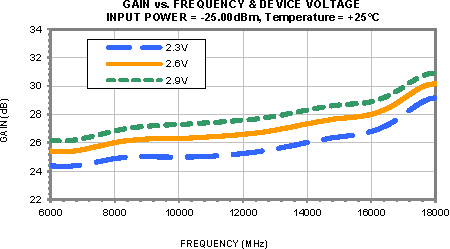
\includegraphics[width=\textwidth]{PMA-GvsFvsV.pdf}
		\caption{}%
		\label{fig:LNA_gain}
	\end{subfigure}
	\hfill
	\begin{subfigure}[b]{0.45\textwidth}
		\centering
		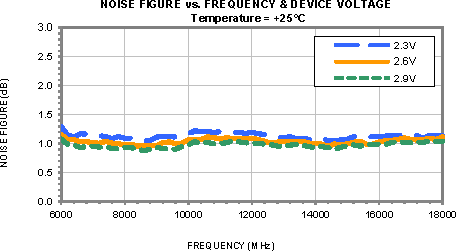
\includegraphics[width=\textwidth]{PMA-NFvsFvsV.pdf}
		\caption{}%
		\label{fig:LNA_NF}
	\end{subfigure}
	\caption{%
		Частотные характеристики:
		(а) усиление при различных напряжениях;
		(б) шум  при различных напряжениях
	}%
	\label{fig:LNA_responses}
\end{figure}


\section{Выбор детектора мощности}

Перст судьбы указывает на \href{https://www.analog.com/en/products/ltc5597.html}{LTC5597} производства Analog Devices. 

Частотные характеристики устройства приведены на Рис.~\ref{fig:LTC_response}.

\begin{figure}[!ht]
		\centering
		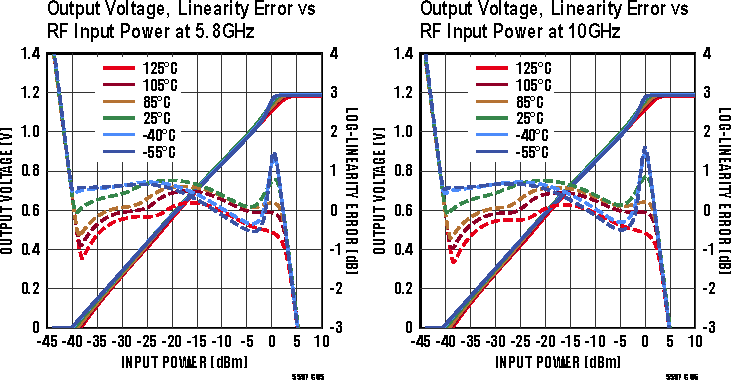
\includegraphics[width=0.9\textwidth]{LTC-power-limits.pdf}
	\caption{Диапазон возможных входных мощностей}%
	\label{fig:LTC_response}
\end{figure}

Основываясь на графиках с  Рис.~\ref{fig:LTC_response} и диапазоне входных мощностей из ТЗ, понимаем, 
что нужно будет ответвлять порядка $-40~\text{дБ}$. 


